\section{Experiment 3 : More Explainable Models}
The results from the previous experiment show that deeper architectures provide higher quality explanations, in other words, their predictions are more explainable. However, there are some cases that the proposed architectures fail to distribute relevance quantities properly.  Hence, this experiment aims to extend the proposed architectures further to address the problem. We consider the same setting as in Section \ref{sec:exp2_prob_formulate}. In the following, we are going to describe three improvement proposals, namely stationary dropout, LSTM-type architecture,  and lateral connections of convolutional layers.


\subsection{Proposal 1 :  Stationary Dropout}
Dropout is a simple regularization technique that randomly suspends the activity of neurons during the training process \citep{SrivastavaDropoutSimpleWay2014} . This randomized suspension allows the neurons to learn better representations and reduces the chance of overfitting.  As a result, it directly influences the quality of explanations.

%\addfigure{\ref{fig:lenet_various_dropout}} shows explanations of LeNet trained with different dropout probability.

%\begin{figure}[!htb]
%\centering
%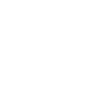
\includegraphics[draft,width=0.5\textwidth]{/sketch/placeholder}
%\caption{LeNet with various dropout values} 
%\label{fig:lenet_various_dropout}  
%\end{figure}



\begin{figure}[!htb]
\centering
\subfloat[Naive Dropout]{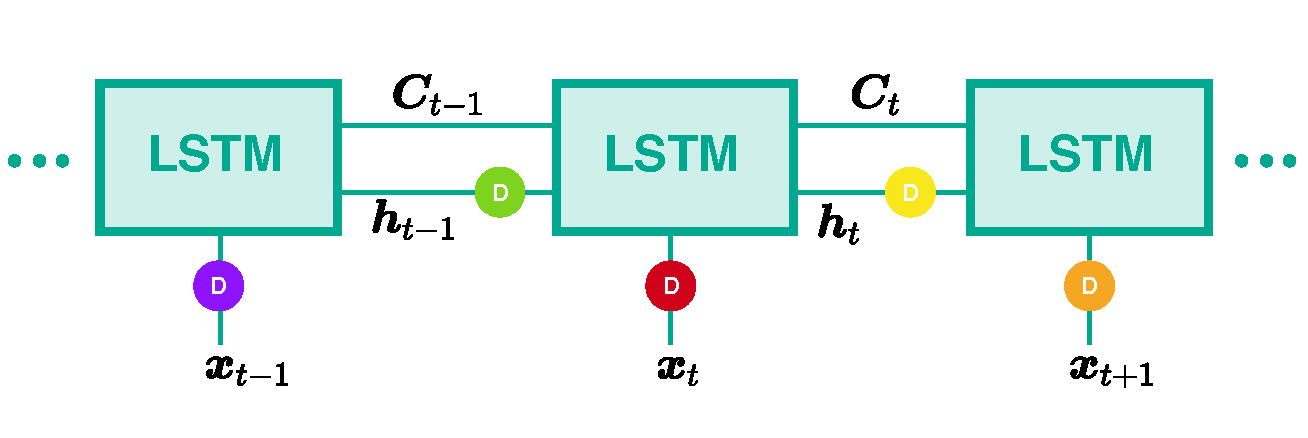
\includegraphics[width=0.45\textwidth]{sketch/lstm_naive_dropout} \label{fig:lstm_naive_dropout}} 
\subfloat[Stationary Dropout]{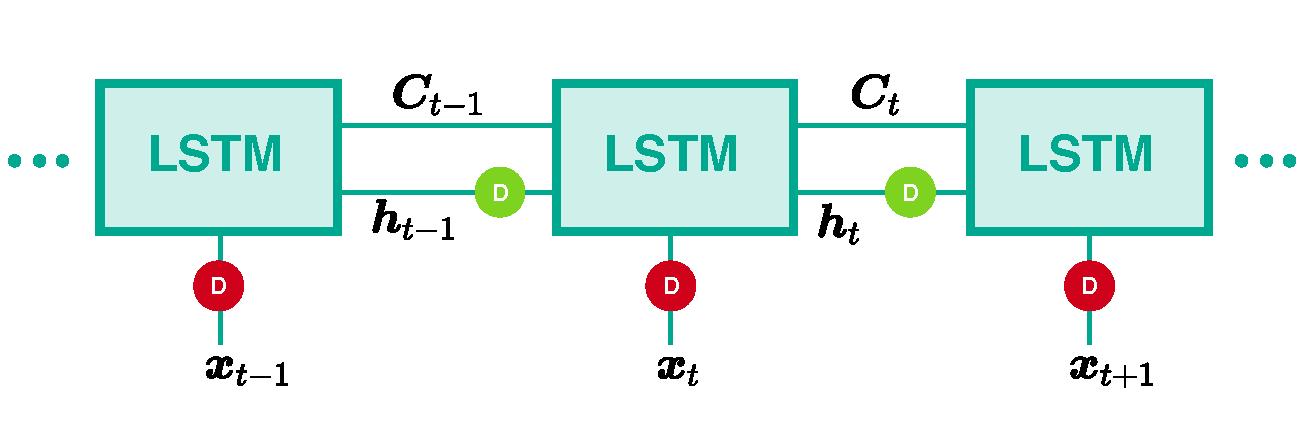
\includegraphics[width=0.45\textwidth]{sketch/lstm_variational_dropout} \label{fig:lstm_variational_dropout}}

\patcaption{LSTM with different dropout approaches.}{\textcircled{\tiny \textbf D} indicates a dropout mask and its color represents a suspending activity. Adapted from \citep{GalTheoreticallyGroundedApplication2016}.}
\label{fig:dropout_lstm}
\end{figure}

Unlike typical feedforward architectures, layers in RNN are shared across time steps. A question arises whether the same neurons in those layers should be suspended or they should be different ones. \addfigure{\ref{fig:dropout_lstm}} illustrates these two different approaches, where different colors represent different suspending activities. In particular, \citet{GalTheoreticallyGroundedApplication2016} proposed and demonstrated that training LSTM and GRU with this stationary dropout approach on language modeling tasks improves accuracy of the models.

%this stationary dropout was first proposed by \citet{GalTheoreticallyGroundedApplication2016} who applied  the technique to LSTM and GRU and found accuracy improvements on language modeling tasks.

\subsection{Proposal 2 : LSTM-type architecture}
\begin{figure}[!htb]
\centering
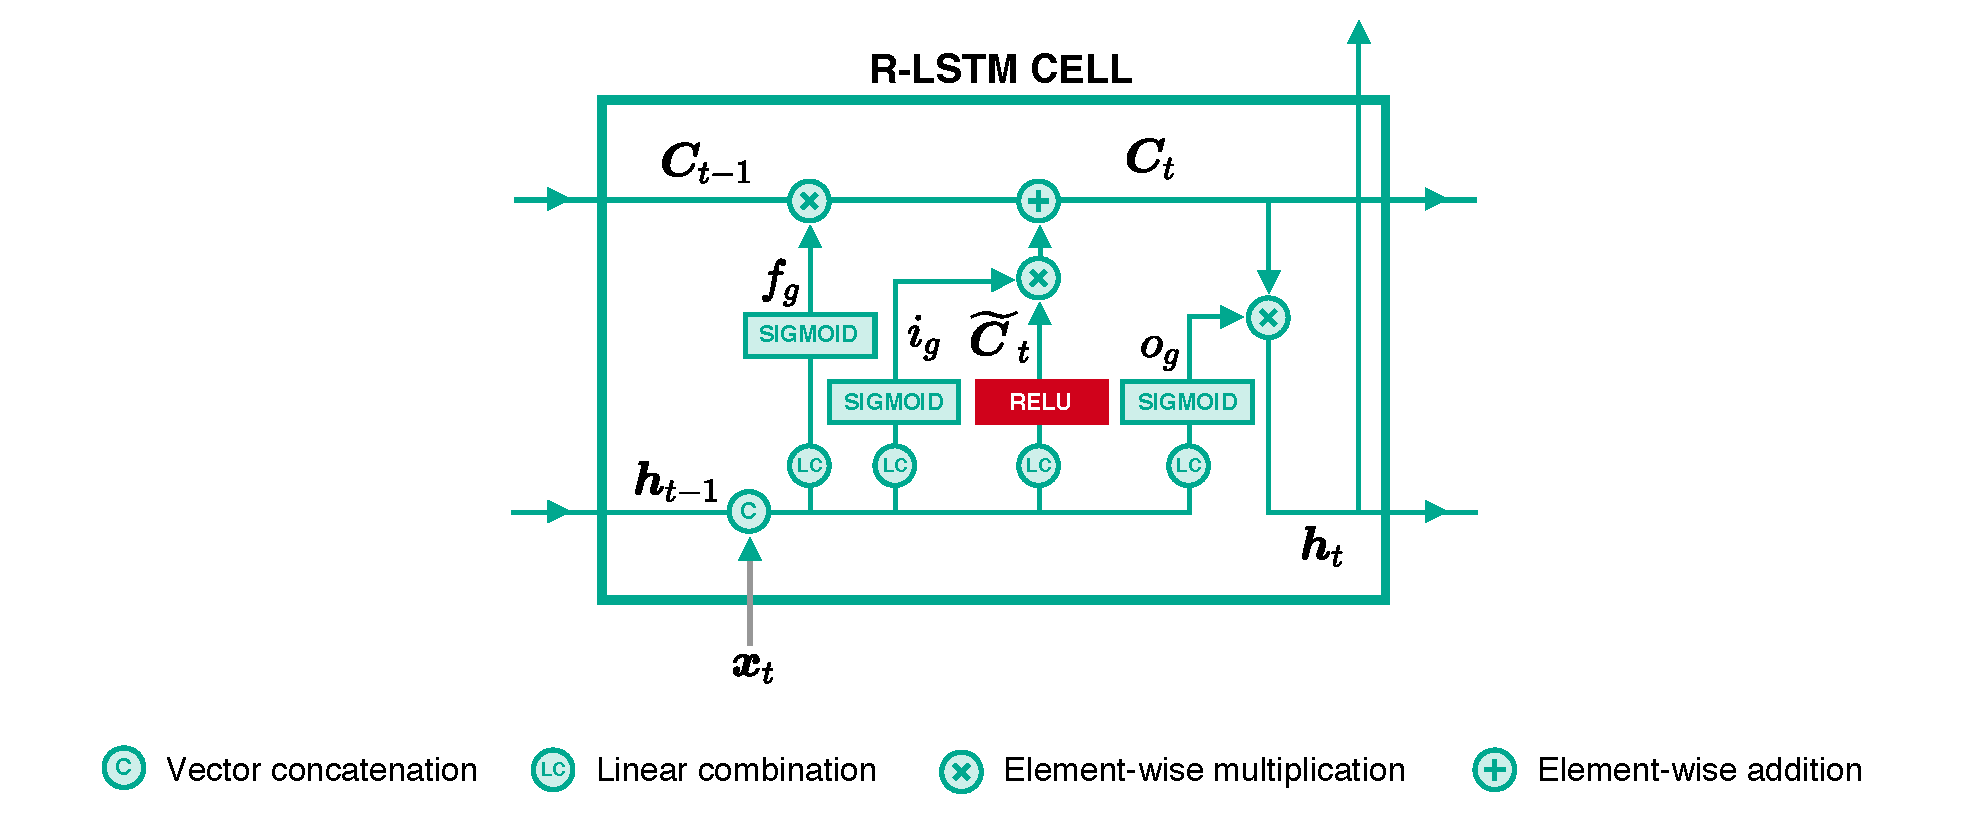
\includegraphics[width=\textwidth]{sketch/relu_lstm}
\caption{R-LSTM structure.} 

\label{fig:relu_lstm} 
\end{figure}

It is already shown that the gating units and the addictive state update are the critical mechanisms that enable LSTM to learn long-term dependencies efficiently \citep{GreffLSTMsearchspace2017, JozefowiczEmpiricalExplorationRecurrent2015}. However, LSTM is not readily applicable to the explanation methods we are considering, except only SA. More precisely, the use of sigmoid and tanh activations violates the assumption of GB and DTD. Therefore, we propose a slightly modified version of LSTM where the ReLU activation is used to compute the  input cell state $\widetilde{C}_t$ instead of the tanh function. This results in $C_t \in \mathbb{R}^+$, hence the tanh activation for $h_t$  is also removed.  As suggested in \citep{ArrasExplainingRecurrentNeural2017},  sigmoid activations are treated as constants when applying DTD and LRP. For GB, we propose to set their partial derivatives to zero. We name this architecture as R-LSTM to differentiate from the original.  \addfigure{\ref{fig:relu_lstm}} presents an overview of the R-LSTM cell.


\subsection{Proposal 3 : Convolutional layer with lateral connections}
We have already seen from the previous experiments that convolution and pooling layers enable NNs to learn hierarchical and invariant representations yielding models with higher accuracy and more explainable predictions. However, the \rnncell{ConvDeep} architecture we proposed in Section \ref{sec:exp2} does not seem to manage to allocate relevance scores to the right input steps in some sequences. We suspect that it is because the architecture has the recurrent mechanism only at the fully-connected layer.


 \begin{figure}
\centering
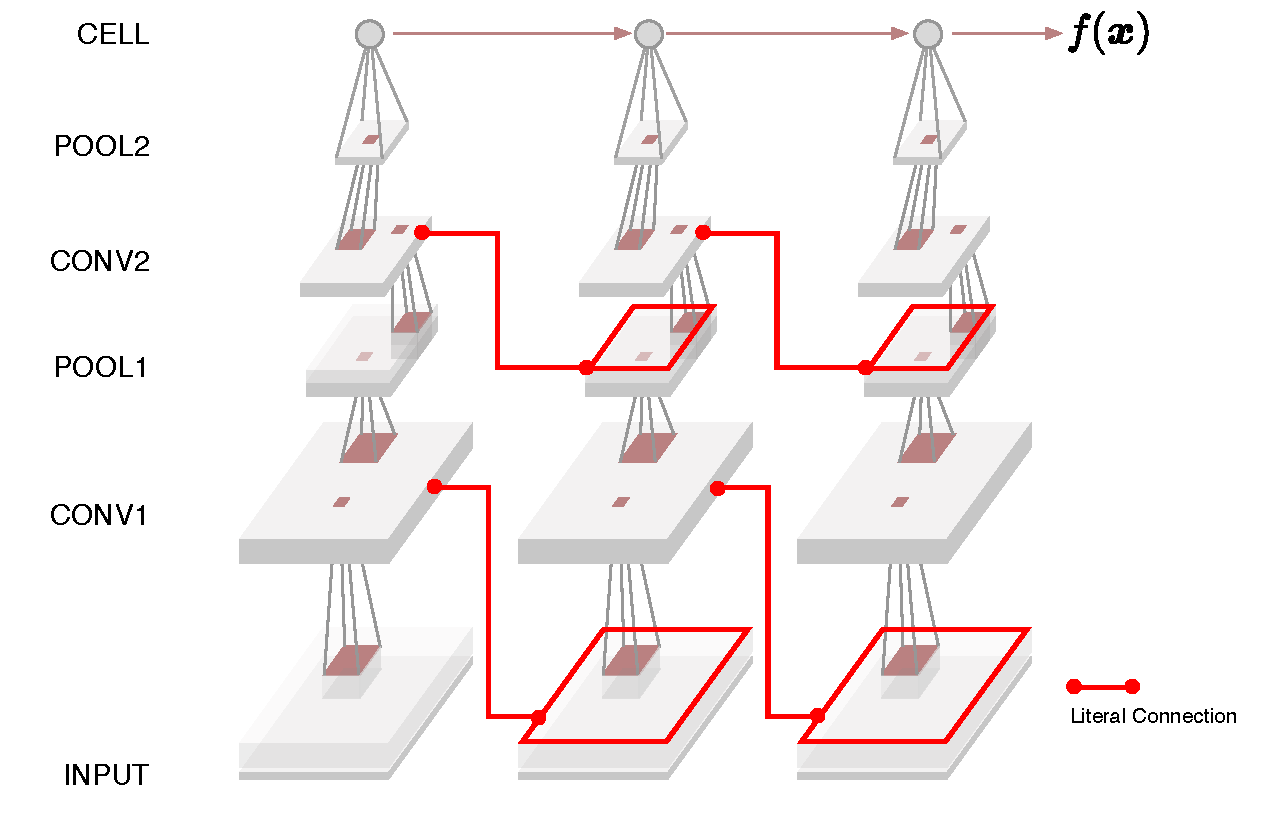
\includegraphics[width=0.9\textwidth]{sketch/conv_literalconn}
\patcaption{ConvDeep with lateral connections (\rnncell{Conv$^+$Deep}).}{} 
\label{fig:conv_literalconn}
\end{figure}

	Therefore, we also propose adding a recurrent mechanism between convolutional operators of each time step. We name these connections as \textit{lateral connections} and \addfigure{\ref{fig:conv_literalconn}} illustrates the connections in red. From the following, we are going to refer Conv$^+$ to the setting that convolutional layers have these  lateral connections.  It is worth mentioning that the connection is possible only when the input and the result of a convolutional operator have the same dimensions.

\subsection{Result}

\begin{figure}
\centering
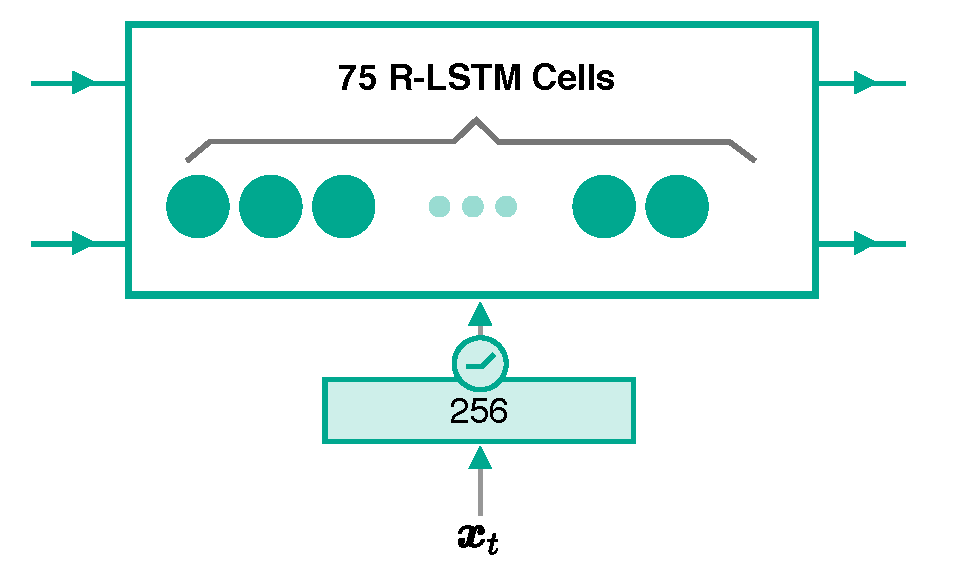
\includegraphics[width=0.5\textwidth]{sketch/r_lstm_setting}
\patcaption{Setting of R-LSTM.}{} 
\label{fig:rlstm_setting}
\end{figure}

In the following, we are going to discuss this experiment in two parts.

In the first part, we will focus on the stationary dropout and R-LSTM proposals. We refer models trained with the stationary dropout approach using the suffix $-SD$. The Deep architecture is used as the baseline.  As can be seen from \addfigure{\ref{fig:rlstm_setting}}, we also introduce a fully-connected layer with 256 neurons between the input layer and the 75 R-LSTM cells to make the configuration of R-LSTM comparable to the Deep architecture.


In the second part, we will discuss the results from the Conv$^+$Deep and ConvR-LSTM-SD architectures. The latter  is simply the R-LSTM-SD architecture that its first fully-connected layer is replaced by convolutions and pooling layers with the same configuration as in ConvDeep. The number of R-LSTM cells is also the same as the first part. ConvDeep and R-LSTM-SD are the baseline architectures for this part.


Table \ref{tab:maj_exp3_model_acc} shows the numbers of trainable parameters in the proposed architectures and accuracies of trained models used for qualitative inspections.

\renewcommand{\arraystretch}{1.5}
\begin{table}[h]
\begin{center}
\patcaption{Numbers of trainable variables and model accuracies of the  proposed architectures in Experiment 3 \trainon.}{The accuracies are computed from the test set.}
\label{tab:maj_exp3_model_acc}
\begin{tabular}{lc|c|c|}
\cline{3-4}
& &
\multicolumn{2}{c|}{\parbox{3.5cm}{ \vskip 1mm \centering \textbf{Accuracy} \vskip 1mm}} \\ \hline
\multicolumn{1}{|l|}{\textbf{Cell architecture}} & \textbf{No. variables} & \textbf{MNIST-MAJ} & \textbf{FashionMNIST-MAJ} \\ \hline
\multicolumn{1}{|l|}{Deep-SD}                  & 153,578             & 98.10\% & 89.47\% \\ 
\multicolumn{1}{|l|}{R-LSTM}                    & 145,701   & 98.50\% & 91.35\% \\ 
\multicolumn{1}{|l|}{R-LSTM-SD}              &  145,701                & 98.57\% & 91.52\% \\ 
 \multicolumn{1}{|l|}{Conv$^+$Deep}       & 175,418                 & 97.92\% & 88.10\% \\
 \multicolumn{1}{|l|}{ConvR-LSTM-SD}      & 152,125                 & 99.35\% & 93.60\%  \\ 
\multicolumn{1}{|l|}{Conv$^+$R-LSTM-SD}   & 175,741                & 98.48\% & 88.19\%  \\ \hline 
\end{tabular}

\end{center}

\end{table}
\renewcommand{\arraystretch}{1}

%todo: mention that Deep is from previous result

\subsubsection{Part 1 : Stationary Dropout and R-LSTM}
 \begin{figure}[!htb]
\centering
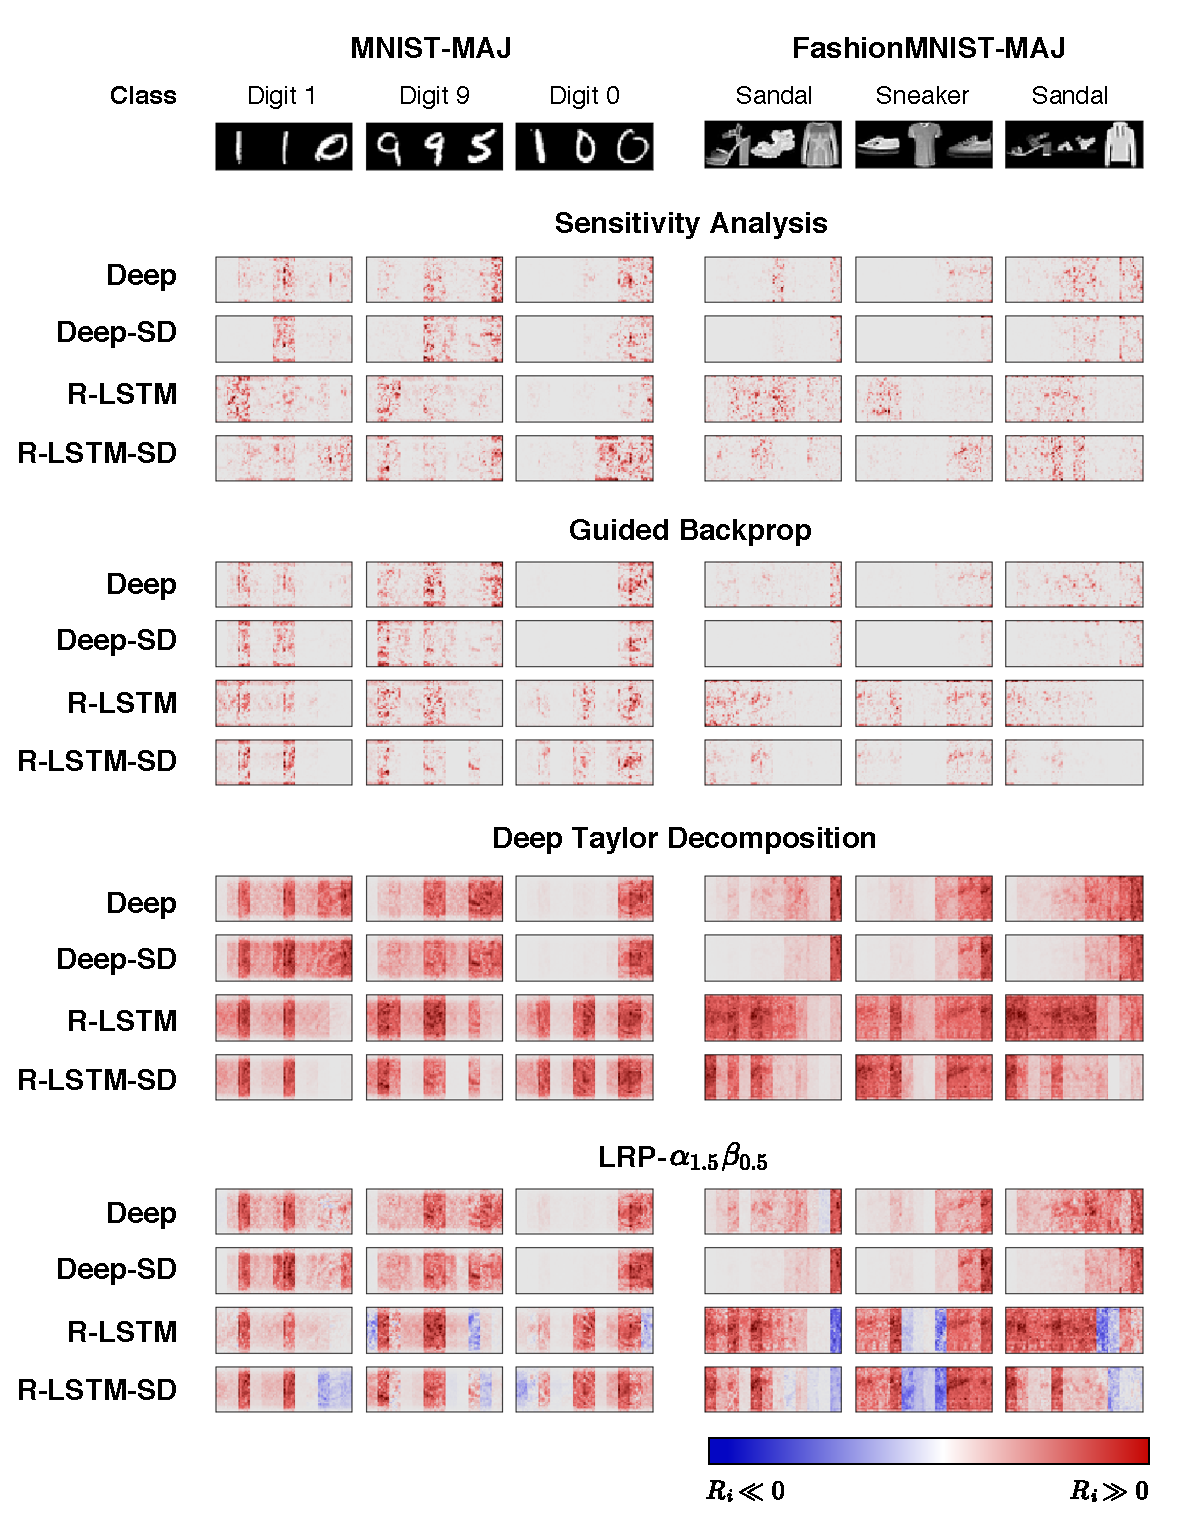
\includegraphics[width=0.8\textwidth]{sketch/heatmap_msc_rlstm_exp}
\patcaption{Relevance heatmaps from different explanation techniques applied to the Deep and R-LSTM architectures \trainon \    using different dropout configurations.}{\heatmapscaleexplain} 
\label{fig:heatmap_msc_rlstm_exp}
\end{figure}

\addfigure{\ref{fig:heatmap_msc_rlstm_exp}} shows the explanation heatmaps from the variants of the Deep and R-LSTM architectures. From the figure, it is apparent that R-LSTM provides considerably better explanations than the Deep architecture on both datasets. We can clearly observe the improvements from the GB, DTD and $\lrpp$ heatmaps. Moreover, training with stationary dropout seems to increase explainability of  R-LSTM. This is well noticeable on the DTD and $\lrpp$ explanations. In contrast, the stationary dropout technique does not seem to have any observable  impact on the explanations of the Deep architecture.


 \begin{figure}[!htb]
\centering
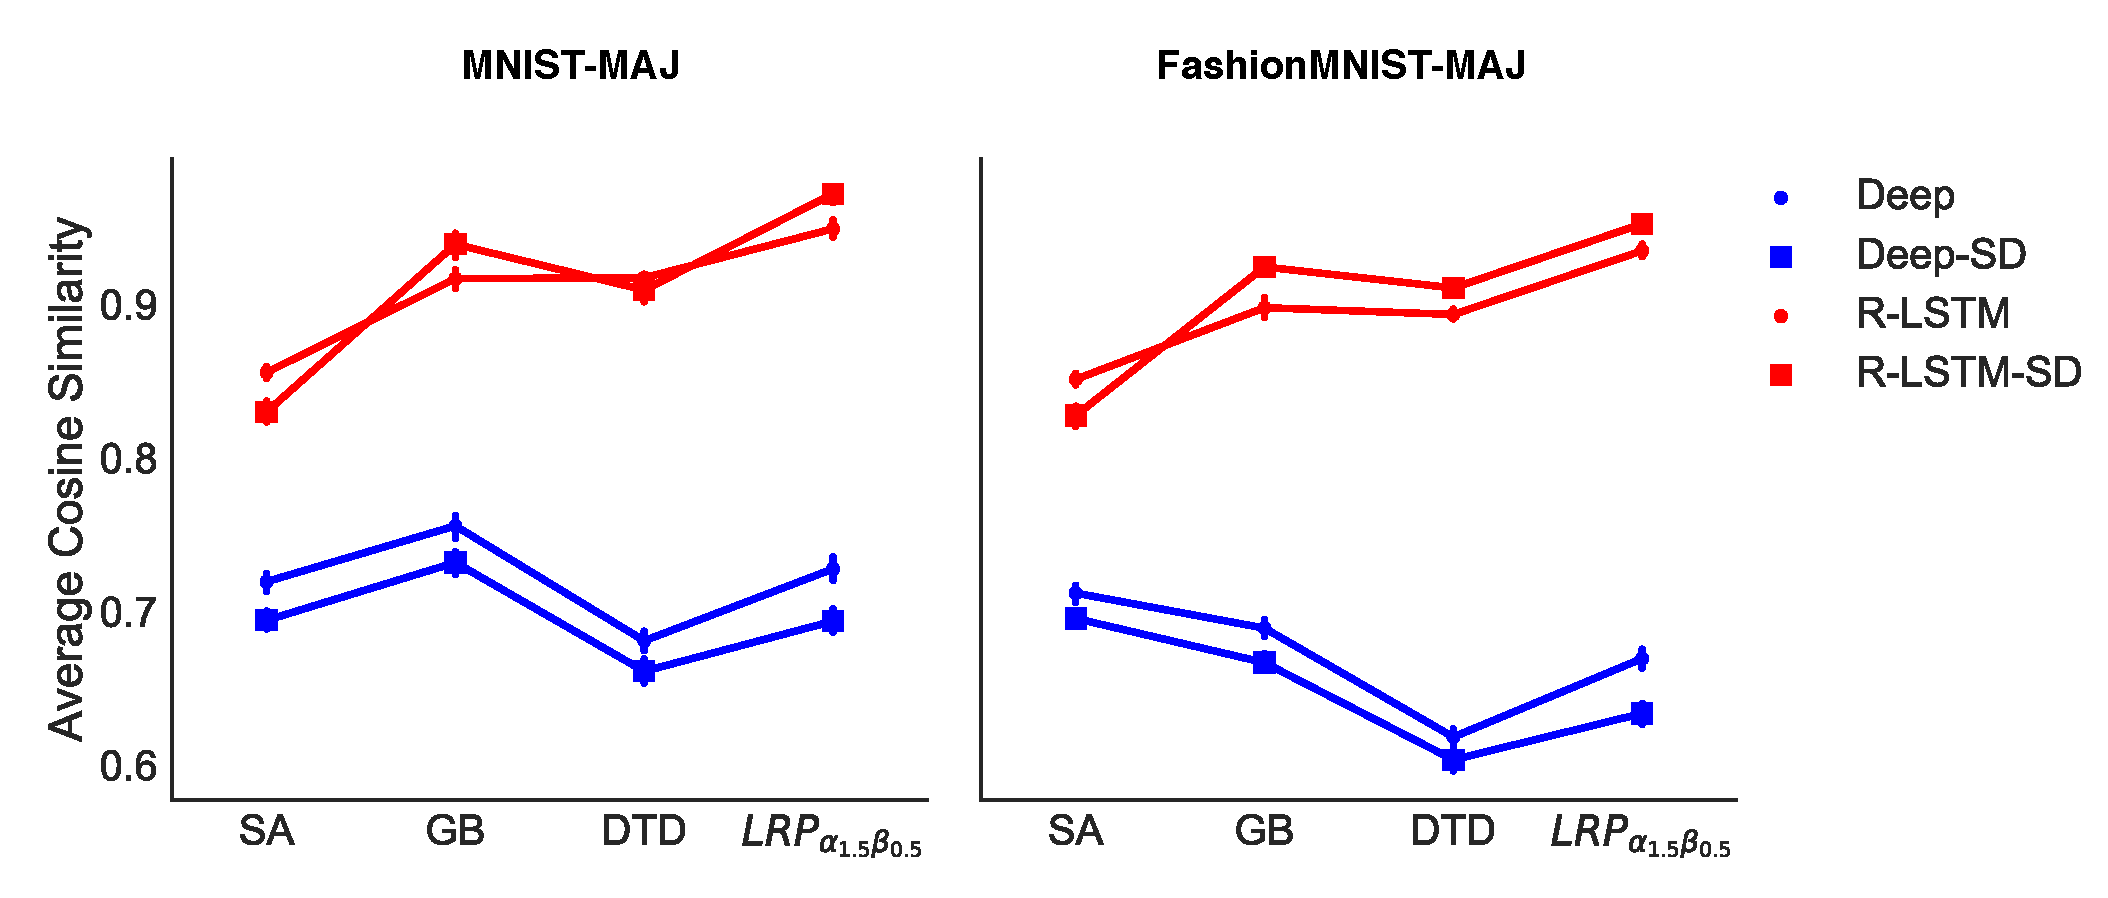
\includegraphics[width=\textwidth]{sketch/rel_dist_rlstm_exp}
%\caption{}  }. 
\patcaption{Cosine similarity measurements from different explanation techniques applied to the Deep and R-LSTM architectures \trainon \ using different dropout configurations.}{The baseline is the Deep architecture depicted by dotted blue line. \quantitativeplotexplain}

\label{fig:rel_dist_rlstm_exp}
\end{figure}

\addfigure{\ref{fig:rel_dist_rlstm_exp}} presents quantitative evaluations of this part. The plots show that  R-LSTM has significantly higher cosine similarity than the Deep architecture regardless of the explanation techniques.  This indicates that R-LSTM is considerably  more explainable than the Deep architecture. Similar to one of the observations in Section \ref{sec:exp1_result}, we also see that the proportion of  the relative cosine similarity improvement from DTD and LRP are slightly higher than the the other methods. This evidence supports the view previously discussed that the DTD and LRP methods are more sensitive to the structure of RNNs.

\addfigure{\ref{fig:rel_dist_rlstm_exp}}  also shows that  R-LSTM trained with stationary dropout (R-LSTM-SD) seems to have better explanations than R-LSTM on every method, except SA. On the other hand, this does not seem to be the case for the Deep architecture. In fact, the plots show that the Deep-SD architecture has notably worse results than the Deep architecture.

%This might be due to more heterogeneous structures in FashionMNIST than MNIST samples. Particularly, we believe that  keeping dropout mask the same for all step would benefit the network to  learn such latent features more efficiently. 
%\todo{hypo thesis?}
%\clearpage

%todo mention that ConvDeep, R-LSTM-SD from previous result
\subsubsection{Part 2 : ConvDeep with lateral connections and ConvR-LSTM-SD}
 \begin{figure}[!htb]
\centering
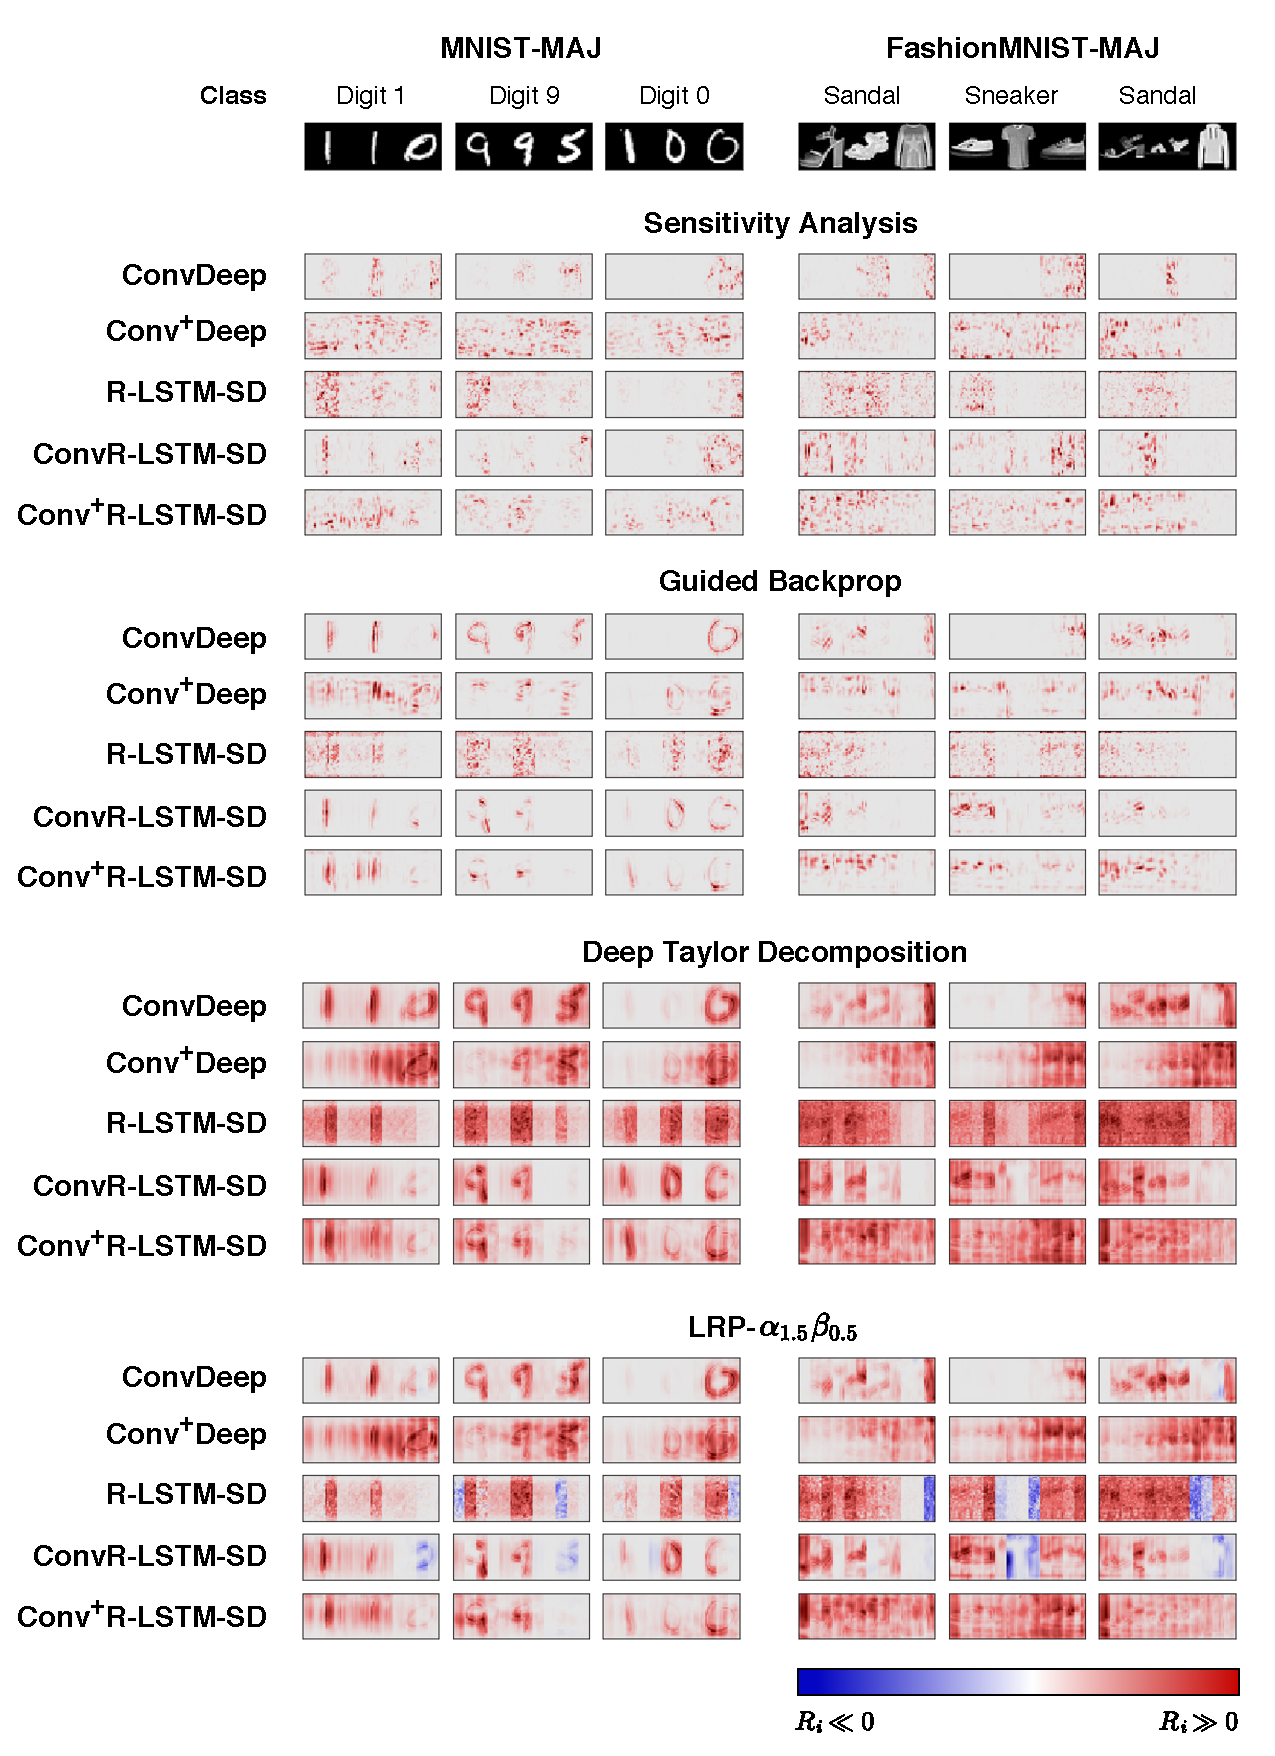
\includegraphics[width=0.8\textwidth]{sketch/heatmap_msc_convtran_exp_v2}
\patcaption{Relevance heatmaps from different explanation techniques applied to variants of ConvDeep and R-LSTM architectures \trainon.}{\heatmapscaleexplain} 
\label{fig:heatmap_msc_convtran_exp}
\end{figure}
For the second part, we are going to discuss results from the ConvDeep with lateral connections (Conv$^+$Deep), and R-LSTM-SD with convolutional and pooling layers (ConvR-LSTM-SD) architectures.

According to \addfigure{\ref{fig:heatmap_msc_convtran_exp}}, Conv$^+$Deep seems to produce worse explanations than the ConvDeep architecture. In particular, this problem is prominent on the DTD and $\lrpp$ explanations. For example, consider Digit 1 and Digit 9 sample, their relevance scores should not have been distributed to the rightmost digit's block. The figure also shows relevance heatmaps from ConvR-LSTM-SD. Comparing to R-LSTM-SD, having convolutional and pooling layers does improve  the quality of the heatmaps further. In particular, we can clearly see the input structures from the explanations.  ConvR-LSTM-SD with lateral connections (Conv$^+$R-LSTM-SD) is also experimented. As expected, the connections reduce the quality of the explanations. This effect is well noticeable on the explanations of the FashionMNIST samples.

\addfigure{\ref{fig:heatmap_msc_convrlstm_pos_rel}} further emphasizes the impact of the convolutional and pooling layers on the R-LSTM-SD architecture. Here, we visualize the relevance heatmaps from the $\lrpp$ method by using only positive scores. We can see that the explanations of ConvR-LSTM-SD are well highlighted and provide substantial features of the input, and more importantly  there are only a small number of the positive scores distributed to non-relevant region.



 \begin{figure}[!htb]
\centering
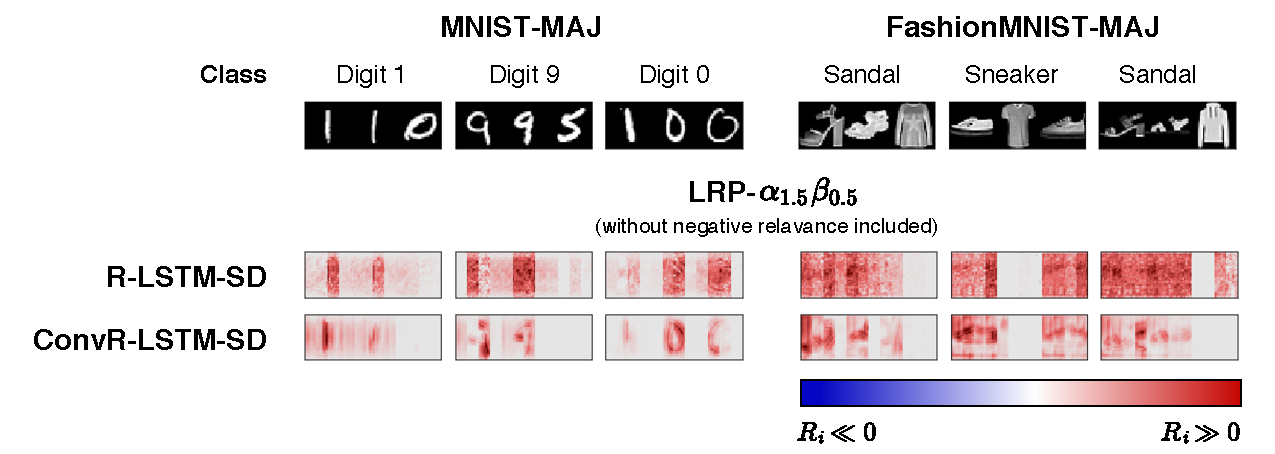
\includegraphics[width=\textwidth]{sketch/heatmap_msc_convrlstm_pos_rel}
\patcaption{Positive relevance heatmaps from $\lrpp$ applied to  the R-LSTM and ConvR-LSTM architectures \trainon.}{\heatmapscaleexplain} 
\label{fig:heatmap_msc_convrlstm_pos_rel}
\end{figure}

 \begin{figure}[!htb]
\centering
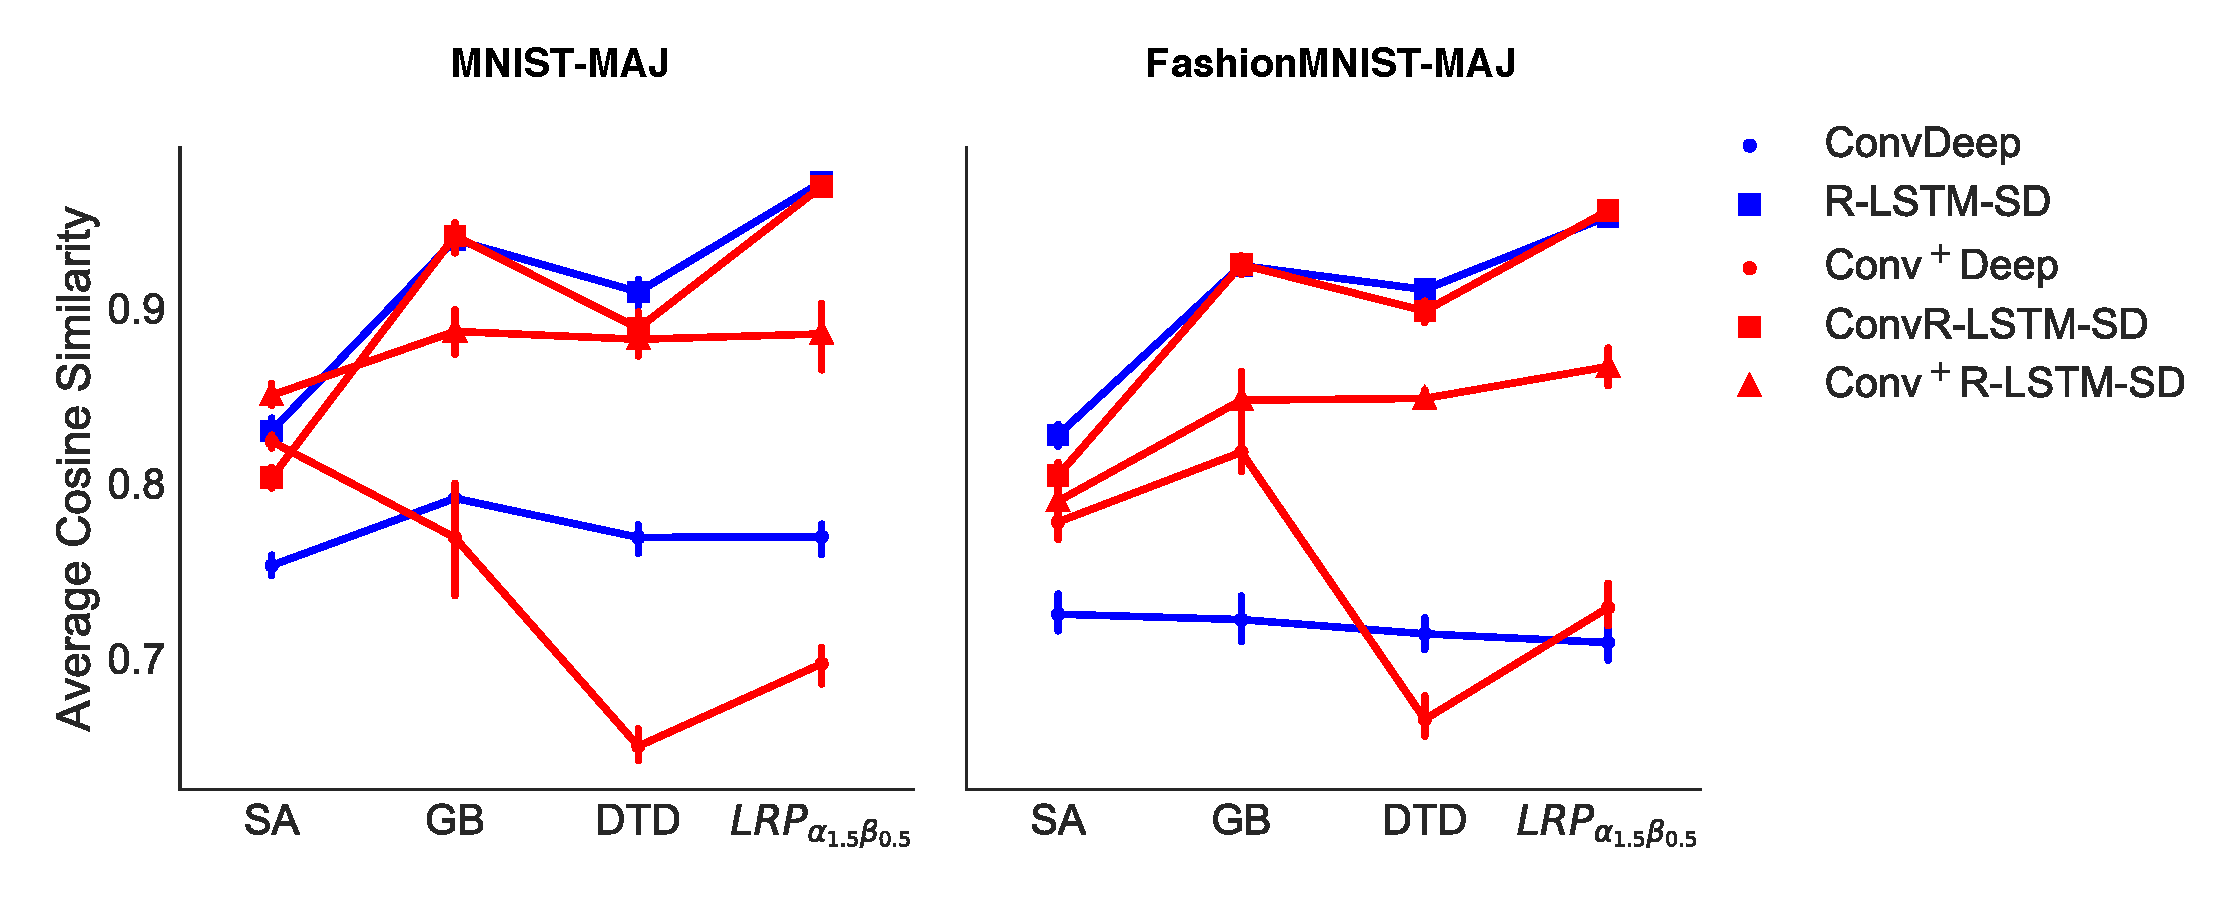
\includegraphics[width=\textwidth]{sketch/rel_dist_convdeep_trans_exp}
\patcaption{Cosine similarity measurements from different explanation techniques applied to variants of the ConvDeep and R-LSTM architectures.}{The ConvDeep and R-LSTM-SD architectures are the baselines presented in blue. \quantitativeplotexplain} 
\label{fig:rel_dist_convdeep_trans_exp}
\end{figure}

\addfigure{\ref{fig:rel_dist_convdeep_trans_exp}} presents the cosine similarity measurements of this second part. Here, the results of the ConvDeep and R-LSTM-SD architectures are the same as the previous experiments. These two architectures are presented here as the baselines, which are presented in blue.  Although,  as shown in \addfigure{\ref{fig:heatmap_msc_convrlstm_pos_rel}}, the explanations of the ConvR-LSTM-SD architecture are less noisy and contain more informative signals corresponding to the input than the R-LSTM-SD architecture, their cosine similarity measurements do not seem to reflect any significant improvement. In fact,  the ConvR-LSTM-SD architecture has lower cosine similarity values from some explanation techniques. We argue that this is a shortcoming of our quantitative measurement because the calculation of the cosine similarity only considers aggregated relevance scores and does not take the smoothness and pixel-wise selectivity of the explanation into account. 

\addfigure{\ref{fig:rel_dist_convdeep_trans_exp}} also show that employing lateral connections in ConvR-LSTM-SD significantly reduces the cosine similarity. This implies that the connections make the models less explainable. On the other hand, the connections in ConvDeep  seem to show an inconsistent influence between MNIST-MAJ and FashionMNIST-MAJ models. 


\subsection{Summary}
We have proposed several improvements to enhance the explainability of RNN models and extensively discussed their results.  Some of which show notable improvements from what we have seen in Section \ref{sec:exp2}. More precisely, using an LSTM-type architecture and training with stationary dropout increase the explainability of RNNs significantly regardless of the explanation techniques.

Moreover, convolutional and pooling layers enable the RNN models to produce more visually understandable explanations than standard fully-connected layers, although this improvement does not seem to be well  captured by our quantitative evaluations. This poses a possible future work in the direction of benchmarking the quality of the explanation.

The lateral connections tend to reduce the explainability of the models.  The connections also seem to make the training process less stable due to the fact that the cosine similarity measurement of the models employing these connections have wider confidence intervals. This is also supported by a decrease in accuracy of the models. 